\section{Durchführung}
\label{sec:Durchführung}

Für den Versuch wird der Aufbau \ref{fig:Bild2} verwendet:
\begin{figure}
	\centering
	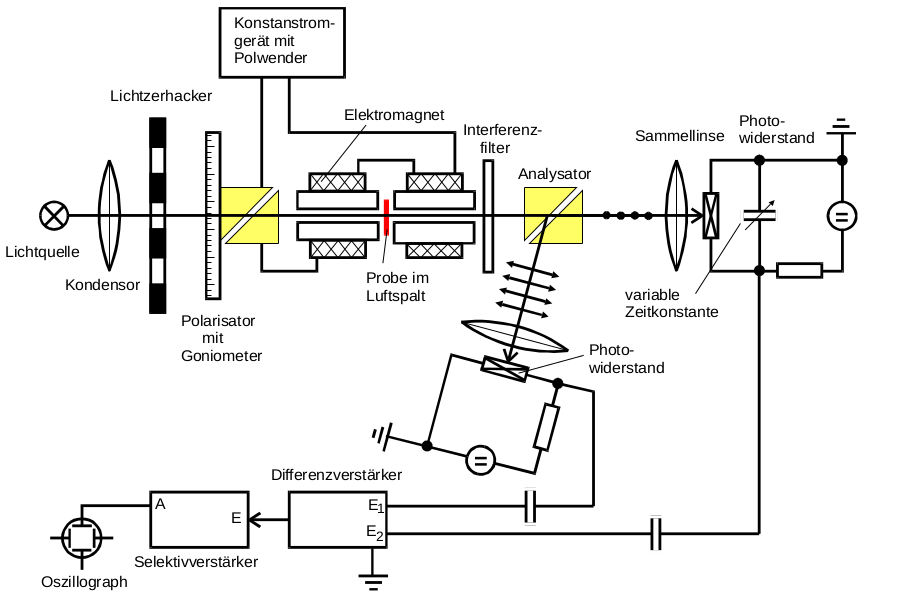
\includegraphics[width=0.8\textwidth]{pictures/aufbau.png}
	\caption{Schematische Darstellung der Messapparatur \cite{Anleitung}}
	\label{fig:Bild2}
\end{figure}
Als Lichtquelle dient eine Halogenlampe mit einem Emissionsspektrum im nahen Infrarotbereich.
Das Licht wird zunächst mittels eines Interferenzfilters monochromatisiert.
Daraufhin passiert es das erste Glan-Thompson-Prisma, welches das Licht linear polarisiert.
Im Mittelpunkt eines großen Elektromagneten befindet sich die zu überprüfende Probe.
Nach dem Austreten aus dem Medium passiert das Licht ein zweites Glan-Thompson-Prisma das,
benötigt wird, um den Drehwinkel $\theta$ zu messen. Die beiden Lichtstrahlen, welche aus dem
Glan-Thompson-Prisma austreten, werden jeweils auf einen Photowiderstand ausgerichtet, um die
Lichtintensität zu messen. An den mit Gleichstrom betriebenen Photowiderständen wird nun in
Abhängigkeit der Lichtintensität ein Spannungsabfall beobachten. Da die Photowiederstände jedoch
einen hohen Innenwiederstand ($\SI{1}{\mega\ohm}$) besitzen, produzieren diese eine
Rauschspannung und es bietet sich so an, in diesem Versuch mit der sogenannten
Wechsellichtmethode zu arbeiten. Dementsprechend wird ein Lichtzerhacker direkt hinter der
Lichtquelle angebracht, der das Licht in Impulse zerhackt. Die an den Photowiederständen
abfallende Wechselspannung wird über einen Kondensator ausgekoppelt und die Differenz der
beiden Strahlen mittels eines Differenzverstärkers ausgerechnet und auf einem Oszilloskop
ausgegeben. Vor dem Oszilloskop wird noch ein auf die Frequenz des Lichtzerhackers abgestimmter
Selektivverstärker angeschlossen. Gibt das Oszilloskop gerade eine Nulllinie aus, so stimmen beide Signale in Betrag und Phase überein.
\subsection{Justierung der Apparatur}
Zuerst wird die Apparatur ohne Medium betrieben und es wird sichergestellt, dass der Lichtstrahl
auf die photosensitiven Flächen des Photowiederstandes trifft. Als nächstes wird die Frequenz
des Lichtzerhackers auf die des Selektivverstärkers eingestellt. Hierzu wird der Lichtzerhacker
in Gang, ein Ausgang am Differenzverstärker auf "Ground" gestellt und das Oszilloskop an den
Ausgang "Resonance" angeschlossen. Dann wird die Frequenz am Selektivverstärker, angefangen
bei der Frequenz des Lichtzerhackers, so eingestellt, dass sich am Oszilloskop ein Maximalstrom
ergibt.
\subsection{Messvorgang}
\begin{itemize}
	\item Um den Drehwinkel des Lichts in einer Probe zu messen wird diese in die Probenhalterung in der Mitte des Elektromagneten gesetzt.
	Der Elektromagnet  wird zuerst auf maximalen Strom eingestellt und das Oszilloskop mittels des Drehwinkels $\theta_1$
		des ersten Glan-Thompson-Prismas auf eine Null-Linie geregelt. Danach wird das
		Feld umgepolt und wieder auf eine Nulllinie gerichtet. Hierbei wird wieder der
		Drehwinkel $\theta_2$ des Prismas am Goniometer abgelesen. Der resultierende
		Drehwinkel ergibt sich also zu:
		\begin{equation*}
			\theta = \frac{1}{2}(\theta_1-\theta_2) \, \mathrm{.}
		\end{equation*}
		Zudem werden acht verschiedene Filter verwendet, um die Faraday-Rotation anhand verschiedener Lichtwellenlängen zu untersuchen.
	\item Am Ende des Experiments wird noch die Kraftflussdichte $B(z)$ in Richtung des
		einfallenden Lichtes mittels einer Hallsonde bei maximalem Feldstrom gemessen.
\end{itemize}
